
%(BEGIN_QUESTION)
% Copyright 2007, Tony R. Kuphaldt, released under the Creative Commons Attribution License (v 1.0)
% This means you may do almost anything with this work of mine, so long as you give me proper credit

Determine the output signal magnitude for each computational relay shown:

$$\includegraphics[width=15.5cm]{i01782x01.eps}$$

\vskip 20pt \vbox{\hrule \hbox{\strut \vrule{} {\bf Suggestions for Socratic discussion} \vrule} \hrule}

\begin{itemize}
\item{} A common problem encountered by students is mistaking the functions of {\it high limit} and {\it high select}, and also {\it low limit} and {\it low select}.  Describe a way to avoid this confusion. 
\end{itemize}

\underbar{file i01782}
%(END_QUESTION)





%(BEGIN_ANSWER)

$$\includegraphics[width=15.5cm]{i01782x02.eps}$$

%(END_ANSWER)





%(BEGIN_NOTES)


%INDEX% Relay, computational: averager function
%INDEX% Relay, computational: limit functions
%INDEX% Relay, computational: selector functions

%(END_NOTES)


